\documentclass[11pt]{article}
\usepackage[margin=1in]{geometry}
\usepackage{tikz}
\usepackage{amsmath,amssymb}
\usepackage{xcolor}
\usetikzlibrary{calc}

\definecolor{tealA}{HTML}{9FE1CB}
\definecolor{tealB}{HTML}{5DCAA5}
\definecolor{tealC}{HTML}{1D9E75}
\definecolor{tealD}{HTML}{0F6E56}
\definecolor{tealE}{HTML}{085041}
\definecolor{coral}{HTML}{D85A30}

\newcommand{\staircase}[2]{%
  \pgfmathtruncatemacro{\kmax}{#1-1}
  \foreach \i in {0,...,\kmax} {
    \pgfmathsetmacro{\xa}{6*(1-\i/#1)}
    \pgfmathsetmacro{\ya}{6*\i/#1}
    \pgfmathsetmacro{\xb}{6*(1-(\i+1)/#1)}
    \pgfmathsetmacro{\yb}{6*(\i+1)/#1}
    \draw[#2, line width=0.9pt] (\xa,\ya) -- (\xb,\ya) -- (\xb,\yb);
  }
}

\title{The staircase paradox:\\ a false proof that $c = a+b$}
\author{}
\date{}

\begin{document}
\maketitle

\section{Setup}

Take a right triangle with legs (catheti) of length $a$ and $b$, and hypotenuse
$c$. Place the right angle at the origin, so the legs run along the axes:
$$(0,0),\qquad (a,0),\qquad (0,b),$$
with the hypotenuse joining $(a,0)$ and $(0,b)$. By Pythagoras,
$c=\sqrt{a^2+b^2}$. For concreteness take $a=b=6$, so $c = 6\sqrt2 \approx 8.485$.

\section{The construction}

Instead of the straight hypotenuse, approximate it by a staircase: replace the
diagonal with a path that alternates horizontal and vertical steps, starting
at $(a,0)$ and ending at $(0,b)$. With $k$ steps, each horizontal segment has
length $a/k$ and each vertical segment has length $b/k$. Figure~\ref{fig:stairs}
shows this staircase for $k = 1,2,4,8,16$, all overlaid on the same triangle,
together with the true hypotenuse in bold.

\begin{figure}[h]
\centering
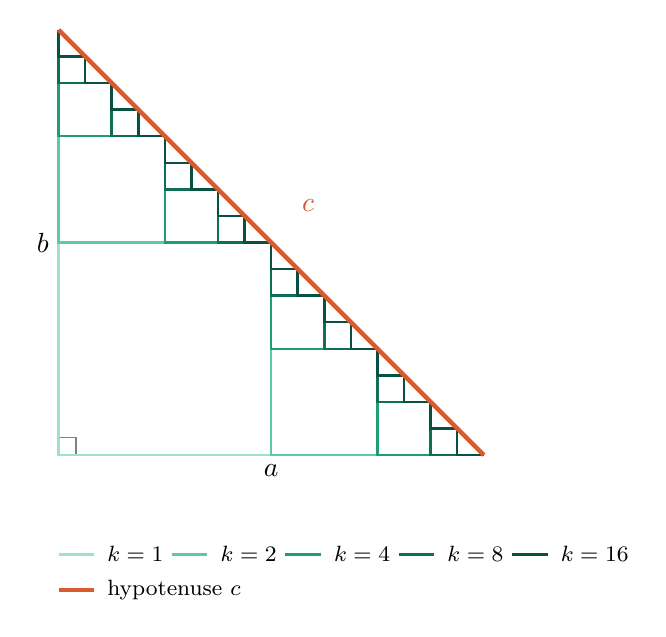
\begin{tikzpicture}[scale=0.9]
  % triangle
  \draw[gray, line width=0.8pt] (0,0) -- (6,0);
  \draw[gray, line width=0.8pt] (0,0) -- (0,6);
  \draw[gray, line width=0.6pt] (0.25,0) -- (0.25,0.25) -- (0,0.25);
  \node[below] at (3,0) {$a$};
  \node[left] at (0,3) {$b$};

  % staircases, coarsest to finest
  \staircase{1}{tealA}
  \staircase{2}{tealB}
  \staircase{4}{tealC}
  \staircase{8}{tealD}
  \staircase{16}{tealE}

  % true hypotenuse
  \draw[coral, line width=1.6pt] (6,0) -- (0,6);
  \node[coral, above right] at (3.3,3.3) {$c$};

  % legend
  \begin{scope}[shift={(0,-1.4)}]
    \draw[tealA, line width=0.9pt] (0,0) -- (0.5,0); \node[right, font=\footnotesize] at (0.55,0) {$k=1$};
    \draw[tealB, line width=0.9pt] (1.6,0) -- (2.1,0); \node[right, font=\footnotesize] at (2.15,0) {$k=2$};
    \draw[tealC, line width=0.9pt] (3.2,0) -- (3.7,0); \node[right, font=\footnotesize] at (3.75,0) {$k=4$};
    \draw[tealD, line width=0.9pt] (4.8,0) -- (5.3,0); \node[right, font=\footnotesize] at (5.35,0) {$k=8$};
    \draw[tealE, line width=0.9pt] (6.4,0) -- (6.9,0); \node[right, font=\footnotesize] at (6.95,0) {$k=16$};
  \end{scope}
  \begin{scope}[shift={(0,-1.9)}]
    \draw[coral, line width=1.6pt] (0,0) -- (0.5,0); \node[right, font=\footnotesize] at (0.55,0) {hypotenuse $c$};
  \end{scope}
\end{tikzpicture}
\caption{Staircases with $k=1,2,4,8,16$ steps between $(a,0)$ and $(0,b)$,
overlaid with the true hypotenuse (coral). As $k$ grows the staircase hugs
the diagonal ever more closely.}
\label{fig:stairs}
\end{figure}

\section{The ``proof''}

For every $k$, the horizontal segments of the staircase sum to exactly $a$
(they partition the base), and the vertical segments sum to exactly $b$.
So the total length of the $k$-step staircase is
$$L_k = a + b,$$
independent of $k$. As $k\to\infty$, the staircase converges pointwise to the
hypotenuse -- every point on it gets arbitrarily close to the diagonal line,
and the maximum distance between the staircase and the line is at most
$\max(a,b)/k \to 0$. Since the staircases ``become'' the hypotenuse in the
limit, and each one has length $a+b$, it seems to follow that
$$c = a+b.$$
For $a=b=6$ this claims $c=12$, in place of the true value $6\sqrt2\approx
8.485$.

\section{Why it fails}

The flaw is the assumption that if a sequence of curves converges to a limit
curve (as point sets, or uniformly), then their lengths converge to the
length of the limit. That assumption is false, and this staircase is the
standard counterexample.

\paragraph{An L1/L2 mismatch.} Every staircase, at any resolution, is a
\emph{taxicab} (L1) path from $(a,0)$ to $(0,b)$: it only ever moves parallel
to the axes. The L1 distance between those two points is exactly $a+b$, and
that number has nothing to do with $k$ -- refining the staircase just
subdivides the same L1 path into smaller axis-aligned pieces, it never turns
it into a diagonal one. The hypotenuse, by contrast, is the L2 (Euclidean)
distance $\sqrt{a^2+b^2}$. No amount of subdividing a taxicab path turns it
into a straight line; you would need to actually tilt the segments, not just
shrink them.

\paragraph{Length is only lower semicontinuous.} What \emph{is} true in
general is
$$\liminf_{k\to\infty} L_k \;\ge\; L(\text{limit curve}),$$
i.e.\ length can jump \emph{up} in the limit but never down -- consistent with
$a+b \ge c$ here (the triangle inequality, with equality only in the
degenerate case $a=0$ or $b=0$). Uniform convergence of curves guarantees
this inequality, not equality. Equality needs more: the curves must converge
together with their \emph{tangent directions} (e.g.\ $C^1$ convergence), so
that each small piece of the approximating curve is not just close to the
limit in position but is pointing the right way. The staircase fails this
badly -- every one of its segments points either due east or due north, never
along the $45^\circ$ direction of the hypotenuse, no matter how small the
steps get.

\section{Conclusion}

The correct statement is Pythagoras' theorem, $c=\sqrt{a^2+b^2}$, not
$c=a+b$. The staircase is a legitimate example of curves that coincide in the
limit as point sets -- the Hausdorff distance between the $k$-step staircase
and the hypotenuse goes to $0$ -- while their lengths stay apart forever,
off by a constant factor of $\dfrac{a+b}{\sqrt{a^2+b^2}}$ (here
$\dfrac{12}{6\sqrt2}=\sqrt2$). It is the same phenomenon as the zig-zag
triangle construction: pointwise or uniform convergence of a sequence of
curves does not, on its own, imply convergence of their lengths.

\end{document}
